\section{Posterior Probability Densities}
\label{appLike}

\begin{figure}[!ht]
  \begin{center}
     \includegraphics[width=0.48\textwidth]{Figures/MCpost1000_6_pe0.pdf}
     \includegraphics[width=0.48\textwidth]{Figures/MCpost1100_6_pe0.pdf}
     \includegraphics[width=0.48\textwidth]{Figures/MCpost1200_6_pe0.pdf}
     \includegraphics[width=0.48\textwidth]{Figures/MCpost1300_6_pe0.pdf}
     \includegraphics[width=0.48\textwidth]{Figures/MCpost1400_6_pe0.pdf}
     \includegraphics[width=0.48\textwidth]{Figures/MCpost1500_6_pe0.pdf}
 \caption{Posterior probability at
 various excited quark resonance masses.  This result include all systematics.
 The 95\% CL upper limit is the value for which 95\% of
 the probability corresponds to smaller cross section: the 95\% quantile.}
    \label{likeli}
  \end{center}
\end{figure}

\clearpage

\begin{figure}[!ht]
  \begin{center}
     \includegraphics[width=0.48\textwidth]{Figures/MCpost1600_6_pe0.pdf}
     \includegraphics[width=0.48\textwidth]{Figures/MCpost1700_6_pe0.pdf}
     \includegraphics[width=0.48\textwidth]{Figures/MCpost1800_6_pe0.pdf}
     \includegraphics[width=0.48\textwidth]{Figures/MCpost1900_6_pe0.pdf}
     \includegraphics[width=0.48\textwidth]{Figures/MCpost2000_6_pe0.pdf}
     \includegraphics[width=0.48\textwidth]{Figures/MCpost2100_6_pe0.pdf}
 \caption{Posterior probability at
 various excited quark resonance masses.  This result include all systematics.
 The 95\% CL upper limit is the value for which 95\% of
 the probability corresponds to smaller cross section: the 95\% quantile.}
    \label{likeli2}
  \end{center}
\end{figure}

\clearpage

\begin{figure}[!ht]
  \begin{center}
     \includegraphics[width=0.48\textwidth]{Figures/MCpost2200_6_pe0.pdf}
     \includegraphics[width=0.48\textwidth]{Figures/MCpost2300_6_pe0.pdf}
     \includegraphics[width=0.48\textwidth]{Figures/MCpost2400_6_pe0.pdf}
     \includegraphics[width=0.48\textwidth]{Figures/MCpost2500_6_pe0.pdf}
     \includegraphics[width=0.48\textwidth]{Figures/MCpost2600_6_pe0.pdf}
     \includegraphics[width=0.48\textwidth]{Figures/MCpost2700_6_pe0.pdf}
 \caption{Posterior probability at
 various excited quark resonance masses.  This result include all systematics.
 The 95\% CL upper limit is the value for which 95\% of
 the probability corresponds to smaller cross section: the 95\% quantile.}
    \label{likeli3}
  \end{center}
\end{figure}

\clearpage

\begin{figure}[!ht]
  \begin{center}
     \includegraphics[width=0.48\textwidth]{Figures/MCpost2800_6_pe0.pdf}
     \includegraphics[width=0.48\textwidth]{Figures/MCpost2900_6_pe0.pdf} 
     \includegraphics[width=0.48\textwidth]{Figures/MCpost3000_6_pe0.pdf}
     \includegraphics[width=0.48\textwidth]{Figures/MCpost3100_6_pe0.pdf}
     \includegraphics[width=0.48\textwidth]{Figures/MCpost3200_6_pe0.pdf}
     \includegraphics[width=0.48\textwidth]{Figures/MCpost3300_6_pe0.pdf}
 \caption{Posterior probability at
 various excited quark resonance masses.  This result include all systematics.
 The 95\% CL upper limit is the value for which 95\% of
 the probability corresponds to smaller cross section: the 95\% quantile.}
    \label{likeli4}
  \end{center}
\end{figure}

\begin{figure}[!ht]
  \begin{center}
     \includegraphics[width=0.48\textwidth]{Figures/MCpost3400_6_pe0.pdf}
     \includegraphics[width=0.48\textwidth]{Figures/MCpost3500_6_pe0.pdf}
     \includegraphics[width=0.48\textwidth]{Figures/MCpost3600_6_pe0.pdf}
     \includegraphics[width=0.48\textwidth]{Figures/MCpost3700_6_pe0.pdf}
     \includegraphics[width=0.48\textwidth]{Figures/MCpost3800_6_pe0.pdf}
     \includegraphics[width=0.48\textwidth]{Figures/MCpost3900_6_pe0.pdf}
 \caption{Posterior probability at
 various excited quark resonance masses.  This result include all systematics.
 The 95\% CL upper limit is the value for which 95\% of
 the probability corresponds to smaller cross section: the 95\% quantile.}
    \label{likeli5}
  \end{center}
\end{figure}

\clearpage

\begin{figure}[!ht]
  \begin{center}
     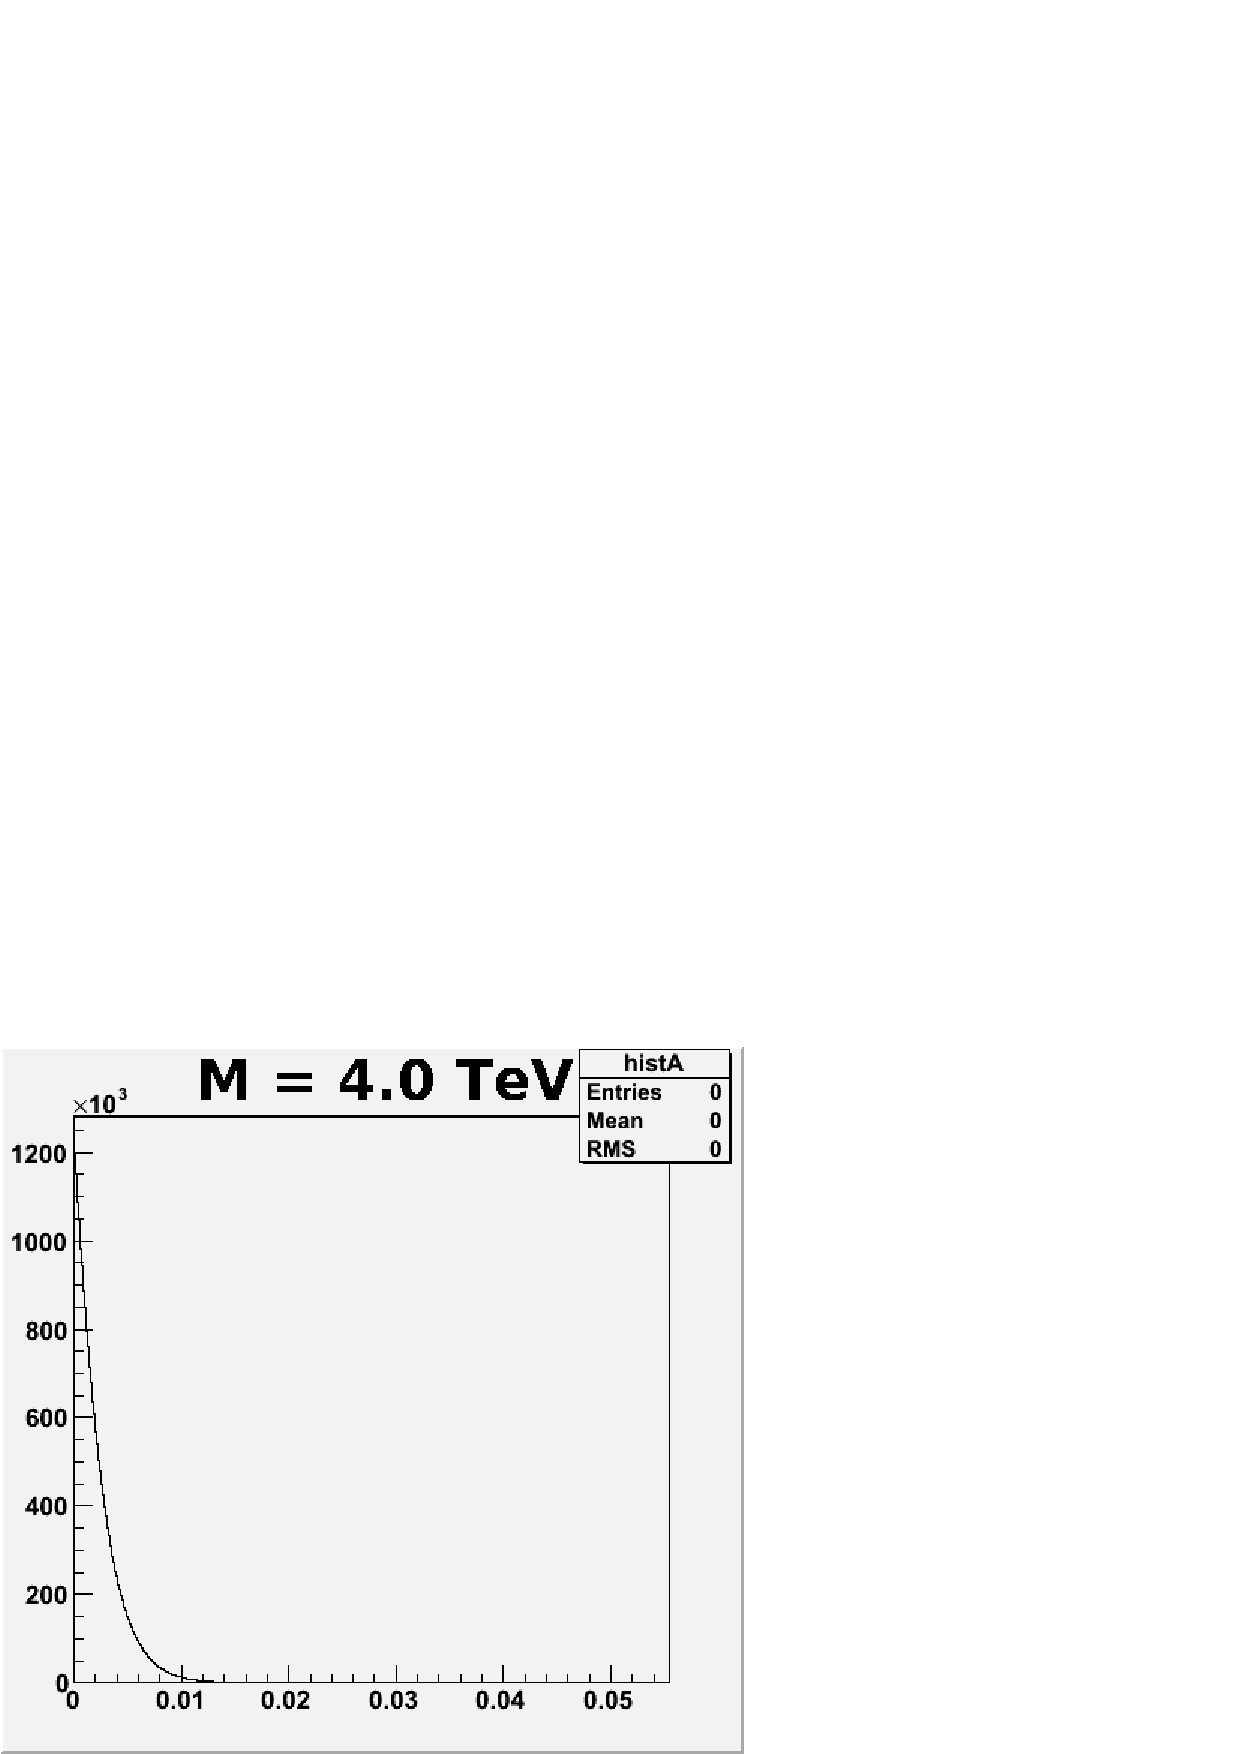
\includegraphics[width=0.48\textwidth]{Figures/MCpost4000_6_pe0.pdf}
     \includegraphics[width=0.48\textwidth]{Figures/MCpost4100_6_pe0.pdf}
 \caption{Posterior probability at
 various excited quark resonance masses. This result include all systematics.
 The 95\% CL upper limit is the value for which 95\% of
 the probability corresponds to smaller cross section: the 95\% quantile.}
    \label{likeli6}
  \end{center}
\end{figure}

\clearpage

\begin{table}[thb]
\centering
       \begin{tabular}{ |c|c|c|c|c|c| }
        \hline
        Resonance & best fit cross section       & best fit cross section      & best fit cross section     \\
	Mass (TeV)& for qq (pb)                  & for qg (pb)                 & for gg (pb)                \\
        \hline
        \hline
        1.0        & $0.00850073\pm0.601313$     & $0.0145012\pm0.615804$      & $0.0212625\pm0.673536$        \\
        \hline
        1.1        & $2.08041e^{-05}\pm0.461261$    & $0.0118713\pm0.528995$      & $0.0408497\pm0.47636$        \\
        \hline
        1.2        & $0.140348\pm0.249355$       & $0.118665\pm0.269844$       & $0.0921535\pm0.310614$   \\
        \hline
        1.3        & $0.0337684\pm0.294504$      & $0.0179412\pm0.292185$      & $0.0336192\pm1.07682$   \\
        \hline
        1.4        & $3.0858e^{-08}\pm0.0785692$    & $7.75251e^{-10}\pm0.0993218$   & $2.15191e^{-09}\pm0.167024$   \\
        \hline
        1.5        & $7.41351e^{-09}\pm0.0745901$   & $8.8934e^{-10}\pm0.0872408$    & $7.99077e^{-12}\pm0.122388$   \\
        \hline
        1.6        & $1.95787e^{-07}\pm0.0769245$   & $1.08725e^{-09}\pm0.0813879$   & $1.01792e^{-09}\pm0.102471$    \\
        \hline
        1.7        & $1.52776e^{-05}\pm0.093486$    & $5.23073e^{-07}\pm0.0969188$   & $4.03072e^{-07}\pm0.15066$      \\
        \hline
        1.8        & $6.20026e^{-08}\pm0.030129$    & $4.57762e^{-08}\pm0.0405528$   & $7.57066e^{-09}\pm0.0656503$   \\
        \hline
        1.9        & $4.01601e^{-07}\pm0.0359546$   & $8.09454e^{-08}\pm0.0444942$   & $3.41376e^{-08}\pm0.0602336$   \\
        \hline
        2.0        & $0.0221219\pm0.0431941$     & $0.0239657\pm0.0559763$     & $0.0242383\pm0.0751805$     \\
        \hline
        2.1        & $0.0126641\pm0.0404499$     & $0.0229555\pm0.0483402$     & $0.0347567\pm0.0636127$     \\
        \hline
	2.2        & $0.0192784\pm0.0323073$     & $0.0265521\pm0.0395536$     & $0.0316009\pm0.05616$     \\
        \hline
	2.3        & $0.0362684\pm0.0301139$     & $0.0445592\pm0.0357687$     & $0.0560383\pm0.0491842$      \\
        \hline
	2.4        & $0.0428054\pm0.0257198$     & $0.0500503\pm0.0307364$     & $0.0660814\pm0.0421347$      \\
        \hline
	2.5        & $0.0346429\pm0.0219307$     & $0.0418594\pm0.0264547$     & $0.058914\pm0.0364333$     \\
        \hline
	2.6        & $0.0157059\pm0.0184392$     & $0.0222136\pm0.022563$      & $0.0321043\pm0.0306874$    \\
        \hline
	2.7        & $0.0072425\pm0.0155485$     & $0.00999937\pm0.0190329$    & $0.0138705\pm0.0250645$    \\
        \hline
        2.8        & $0.00950811\pm0.0129434$    & $0.0101158\pm0.0158875$     & $0.0122459\pm0.0211184$   \\
        \hline
        2.9        & $0.00716419\pm0.0108225$    & $0.00721799\pm0.0128416$    & $0.00904771\pm0.0173866$   \\
        \hline
        3.0        & $0.00145038\pm0.00669575$   & $0.000591449\pm0.012469$    & $0.00111588\pm0.0192463$     \\
        \hline
        3.1        & $3.35651e^{-11}\pm0.00391246$  & $2.74513e^{-10}\pm0.00550929$  & $4.26457e^{-10}\pm0.00901187$        \\
        \hline
        3.2        & $7.43403e^{-10}\pm0.00195856$  & $1.03111e^{-08}\pm0.00277021$  & $3.29472e^{-08}\pm0.00428968$   \\
        \hline
        3.3        & $3.27862e^{-08}\pm0.00153612$  & $1.54421e^{-08}\pm0.00195851$  & $1.01819e^{-13}\pm0.00285528$   \\
        \hline
        3.4        & $2.58143e^{-08}\pm0.00127592$  & $4.04395e^{-08}\pm0.00169161$  & $2.03405e^{-08}\pm0.00240395$   \\
        \hline
        3.5        & $4.00802e^{-14}\pm0.00120312$  & $6.50918e^{-14}\pm0.00157685$  & $1.58561e^{-07}\pm0.00225683$   \\
        \hline
        3.6        & $2.65408e^{-12}\pm0.00123848$  & $5.6704e^{-13}\pm0.00157895$   & $1.54178e^{-07}\pm0.00212173$    \\
        \hline
        3.7        & $1.16325e^{-10}\pm0.00137765$  & $2.76524e^{-13}\pm0.00168705$  & $2.28831e^{-08}\pm0.00215576$      \\
        \hline
        3.8        & $3.58264e^{-13}\pm0.00138734$  & $4.00608e^{-12}\pm0.00171275$  & $4.2247e^{-07}\pm0.0022446$   \\
        \hline
        3.9        & $1.05284e^{-10}\pm0.00108164$  & $5.03204e^{-14}\pm0.00139058$  & $4.92234e^{-08}\pm0.00179093$   \\
        \hline
        4.0        & $1.86222e^{-08}\pm0.000934835$ & $1.63525e^{-07}\pm0.00121964$  & $2.30862e^{-07}\pm0.00156344$     \\
        \hline
        4.1        & $2.03997e^{-10}\pm0.000866091$ & $1.21219e^{-08}\pm0.00108286$  & $5.72931e^{-10}\pm0.00132742$     \\
        \hline
       \end{tabular}
       \caption{Best cross section values from fit for each resonance mass.}
       \label{likeli_best_xs}
\end{table}

